\documentclass{reportOpenlab} % custom style based on LaTeX article
\addbibresource{bibliography.bib} % path to bibliography file

\begin{document}

%--------------------- Define project ------------------------
\title{Full Title of the Report}
\author{First Name Family Name of the Author}
\institute{XYZ Competence Centre etc.}
\supervisor{First Name Family Name\\First Name Family Name etc.}
\date{MONTH 2022}
\reportnumber{x/2022}

%--------------------- Produce first pages ------------------------
\maketitlepage

\specification{Your Project Specification goes here.}

\abstract{Abstract of your Report.}

\tableofcontents

%--------------------- Include main content ------------------------

\markdownInput{README.md} % Example on how to include markdown

\subsection{More}

More information on how to include content of markdown files is available for instance at \url{https://www.overleaf.com/learn/how-to/Writing_Markdown_in_LaTeX_Documents}

\section{INTRODUCTION}
Introduction to your project.

\begin{figure}[h]
\centering
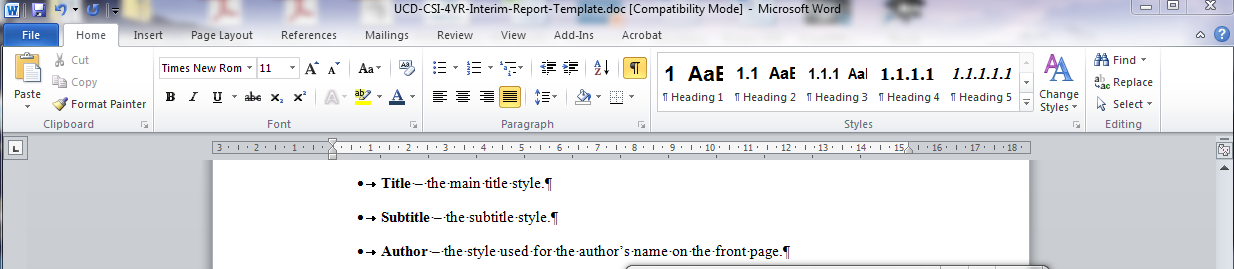
\includegraphics[width=0.5\textwidth]{assets/example.png}
\caption{Example of a figure~\cite{exampleCitation}}
\label{fig:example}
\end{figure}

Example is presented in Fig.~\ref{fig:example}.

More information is available for instance at \url{https://www.overleaf.com/learn/latex/Inserting_Images}.

\section{TWO}
Another section.

\begin{listing}[!ht]
\begin{minted}[highlightlines={3}]{python}
import numpy as np
    
def incmatrix(genl1,genl2):
    m = len(genl1)
    n = len(genl2)
    M = None #to become the incidence matrix
    VT = np.zeros((n*m,1), int)  #dummy variable
    
    #compute the bitwise xor matrix
    M1 = bitxormatrix(genl1)
    M2 = np.triu(bitxormatrix(genl2),1) 

    for i in range(m-1):
        for j in range(i+1, m):
            [r,c] = np.where(M2 == M1[i,j])
            for k in range(len(r)):
                VT[(i)*n + r[k]] = 1;
                VT[(i)*n + c[k]] = 1;
                VT[(j)*n + r[k]] = 1;
                VT[(j)*n + c[k]] = 1;
                
                if M is None:
                    M = np.copy(VT)
                else:
                    M = np.concatenate((M, VT), 1)
                
                VT = np.zeros((n*m,1), int)
    
    return M
\end{minted}
\caption{Example code snippet~\cite{code}.}
\end{listing}

More information on code snippets is available for instance at:
\begin{itemize}
    \item \url{https://www.overleaf.com/learn/latex/Code_Highlighting_with_minted},
    \item \href{https://repo.skni.umcs.pl/ctan/macros/latex/contrib/minted/minted.pdf}{Package documentation.}
\end{itemize}

\section*{REFERENCES}
\printbibliography[heading=none]

More information on bibliography is available for instance at \url{https://www.overleaf.com/learn/latex/Bibliography_management_with_biblatex}.}}

\end{document}